% ---------
%  Compile with "pdflatex hw0".  
% --------
%!TEX TS-program = pdflatex

\documentclass[11pt]{article}
\usepackage{jeffe,handout,graphicx}

% ---------
% Input file uses Unicode's UTF-8 encoding
% ---------
%!TEX encoding = UTF-8 Unicode
\usepackage[utf8]{inputenc}

% ---------
%  The next several lines (up to the line of =='s) change the default text
%  and math fonts and make a few other minor cosmetic changes.  If you get
%  any error messages related to these packages, just comment them out.
%         -- Jeff
% --------
\usepackage[charter]{mathdesign}
\def\sfdefault{fvs}
\def\ttdefault{fvm}
\SetMathAlphabet{\mathsf}{bold}{\encodingdefault}{\sfdefault}{b}{\updefault}
\SetMathAlphabet{\mathtt}{bold}{\encodingdefault}{\ttdefault}{b}{\updefault}
\SetMathAlphabet{\mathsf}{normal}{\encodingdefault}{\sfdefault}{\mddefault}{\updefault}
\SetMathAlphabet{\mathtt}{normal}{\encodingdefault}{\ttdefault}{\mddefault}{\updefault}
\usepackage{microtype}
% ---------
%  End of cosmetics.
% --------

% ---------
%  Redefine suits
% --------
\usepackage{pifont}
\def\Spade{\ding{171}}
\def\Heart{\textcolor{Red}{\ding{170}}}
\def\Diamond{\textcolor{Red}{\ding{169}}}
\def\Club{\ding{168}}

% =========================================================
\begin{document}

\headers{CS 573}{Homework 0 (due September 1, 2010)}{Fall 2010}

\begin{center}
\LARGE
\textbf{CS 573: Graduate Algorithms, Fall 2010}
\\
\textbf{Homework 0}
\\[1ex]
\Large
Due Wednesday, September 1, 2010 \underline{\textbf{in class}}
\end{center}

\hrule

\begin{itemize}

\item
This homework tests your familiarity with prerequisite material (\url{http://www.cs.uiuc.edu/class/fa10/cs573/stuff-you-already-know.html}) to help you identify gaps in your background knowledge.  \textbf{You are responsible for filling those gaps.}  Fr most topics, the early chapters of any algorithms textbook should be sufficient review, but you may also want consult your favorite discrete mathematics and data structures textbooks.  If you need help, please ask in office hours and/or on the course newsgroup.

\item
Each student must submit individual solutions for these homework problems.  For all future homeworks, groups of up to three students may submit (or present) a single group solution for each problem.

\item
Please carefully read the course policies linked from the course web site.  If you have \emph{any} questions, please ask during lecture or office hours, or post your question to the course newsgroup.  In particular:
\begin{itemize}
\item
Submit five separately stapled solutions, one for each numbered problem, with your name and NetID clearly printed on each page.  Please do \emph{not} staple everything together.
\item
You may use any source at your disposal---paper, electronic, or human---but you \EMPH{must} write your solutions in your own words, and you \EMPH{must} cite every source that you use.  In particular, each solution should include a list of \emph{everyone} you worked with to solve that problem.
\item
Unless explicitly stated otherwise, \EMPH{every} homework problem requires a proof.
\item
Answering ``I don't know'' to any homework or exam problem (except for extra credit problems) is worth 25\% partial credit.
\item
Algorithms or proofs containing phrases like ``and so on'' or ``repeat this process for all $n$'' instead of an explicit loop, recursion, or induction, will receive 0 points.
\end{itemize}

\end{itemize}

\hrule

\newpage
\begin{enumerate}
\parindent 1.5em \itemsep 4ex plus 0.5fil

\item
\begin{enumerate}\itemsep 2ex plus 0.1fil
\item[(•)]
\textcolor{red}{\EMPH{Write the sentence ``I understand the course policies."}}

Solutions that omit this sentence will not be graded.

\item
\textbf{[5 pts]}
Solve the following recurrences.  State tight asymptotic bounds for each function in the form $\Theta(f(n))$ for some recognizable function $f(n)$.  Assume reasonable but nontrivial base cases if none are given.  \EMPH{Do not submit proofs}---just a list of five functions---but you should do them anyway, just for practice.
\medskip
\begin{itemize}\itemsep 1ex
\item
$A(n) = 4\,A(n-1) + 1$
\item
$B(n) = B(n-3) + n^2$
\item
$C(n) = 2\, C(n/2) + 3\, C(n/3) + n^2$
\item
$D(n) = 2\, D(n/3) + \sqrt{n}$
\item
$E(n) = \begin{cases}
	n & \text{if $n\le 3$,} \\[1.5ex]
	\Frac{E(n-1)E(n-2)}{E(n-3)} & \text{otherwise}
\end{cases}$\qquad
\Hint{This is easier than it looks!}
\end{itemize}


\item
\textbf{[5 pts]}
Sort the following functions from asymptotically smallest to asymptotically largest, indicating ties if there are any.   \EMPH{Do not submit proofs}---just a sorted list of 16 functions---but you should do them anyway, just for practice.

\quad Write $f(n) \ll g(n)$ to indicate that $f(n) = o(g(n))$, and write $f(n) \equiv g(n)$ to mean $f(n) = \Theta(g(n))$.  We use the notation $\lg n = \log_2 n$.

\[
\mfbox{
\begin{array}{c@{\quad}c@{\quad}c@{\quad}c}
		n &
		\lg n &
		\sqrt{n}  &
		7^n
	\\[2ex]
		\sqrt{\lg n} &
		\lg \sqrt{n} &
		7^{\sqrt{n}}  &
		\sqrt{7^n}
	\\[2ex]
		7^{\lg n} &
		\lg(7^n) &
		7^{\lg \sqrt{n}} &
		7^{\sqrt{\lg n}} 
	\\[2ex]
		\sqrt{7^{\lg n}} &
		\lg (7^{\sqrt{n}})  &
		\lg \sqrt{7^n}  &
		\sqrt{\lg (7^n)}
\end{array}}
\]

\end{enumerate}

%----------------------------------------------------------------------
\def\symbol#1{\textbf{\texttt{#1}}}

\item
Professore Giorgio della Giungla has a 23-node binary tree, in which every node is labeled with a unique letter of the Roman alphabet, which is just like the modern English alphabet, but without the letters \symbol{J}, \symbol{U}, and \symbol{W}.  Inorder and postorder traversals of the tree visit the nodes in the following order:
\begin{itemize}
\item
	\mbox{\hbox to 0pt{Inorder:\hss}\phantom{Postorder: }}%
	\symbol{S V Z A T P R D B X O L F E H I Q M N G Y K C}
\item Postorder:
	\symbol{A Z P T X B D L E F O H R I V N M K C Y G Q S}
\end{itemize}

\begin{enumerate}
\item
List the nodes in Prof. della Giungla's tree in the order visited by a \emph{preorder} traversal. 

\item
Draw Prof. della Giungla's tree.

\end{enumerate}

%----------------------------------------------------------------------
\newpage
\item
\textcolor{Red}{\textsf{The original version of this problem asked to support the mirror-image operations \textsc{\textrm{LowestToRight}} and \textsc{\textrm{LeftmostAbove}}, which are \emph{much} harder to support with a single data structure that stores each point at most once.  We will accept $O(n)$-space data structures for either version of the problem for full credit.}}

Describe a data structure that stores a set $S$ of $n$ points in the plane, each represented by a pair $(x,y)$ of coordinates, and supports the following queries.
\begin{itemize}
\item
\EMPH{\textsc{HighestToRight}$(\ell)$:} Return the highest point in $S$ whose $x$-coordinate is greater than or equal to $\ell$.  If every point in $S$ has $x$-coordinate less than $\ell$, return \textsc{None}.
\item
\EMPH{$\textsc{RightmostAbove}(\ell)$:}  Return the rightmost point in $S$ whose $y$-coordinate is greater than or equal to $\ell$.  If every point in $S$ has $y$-coordinate less than $\ell$, return \textsc{None}.
\end{itemize}
%
For example, if $S = \Set{(3,1),~ (1,9),~ (9,2),~ (6,3),~ (5,8),~ (7,5),~ (4,10),~ (0,7)}$, then both \textsc{HighestToRight}$(4)$ and \textsc{RightmostAbove}$(6)$ should return the point $(5,8)$, and \textsc{HighestToRight}$(10)$ should return \textsc{None}.

\begin{inline}
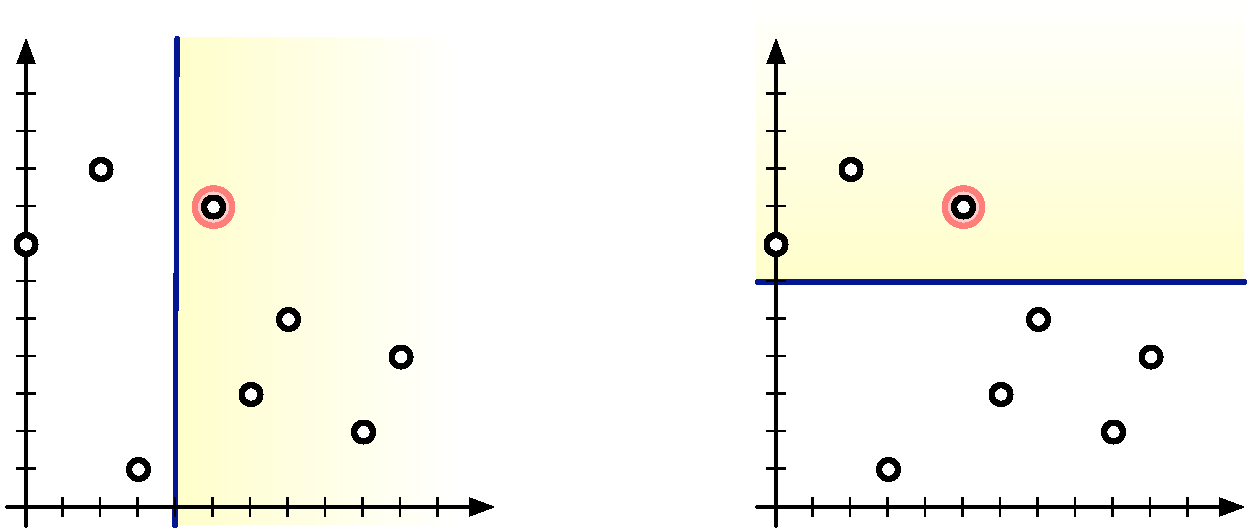
\includegraphics[height=1.5in]{Fig/rightabove}\\
$\textsc{\textrm{HighestToRight}}(4) = \textsc{\textrm{RightmostAbove}}(6) = (5,8)$
\end{inline}

Analyze both the size of your data structure and the running times of your query algorithms.  For full credit, your data structure should use $O(n)$ space, and each query algorithm should run in $O(\log n)$ time.  \textcolor{Red}{\EMPH{For 5 extra credit points, describe a data structure that stores each point at most once.}}  You may assume that no two points in $S$ have equal $x$-coordinates or equal $y$-coordinates.

\Hint{Modify one of the standard data structures listed at \url{http://www.cs.uiuc.edu/class/fa10/cs573/stuff-you-already-know.html}, but just describe your changes; don't regurgitate the details of the standard data structure.}


%----------------------------------------------------------------------
\item
An \EMPH{arithmetic expression tree} is a binary tree where every leaf is labeled with a variable, every internal node is labeled with an arithmetic operation, and every internal node has exactly two children.  For this problem, assume that the only allowed operations are $\mathbs{+}$ and $\mathbs{\times}$.  Different leaves may or may not represent different variables.

Every arithmetic expression tree represents a function, transforming input values for the leaf variables into an output value for the root, by following two simple rules:  (1) The value of any $+$-node is the sum of the values of its children.  (2) The value of any $\times$-node is the product of the values of its children.

Two arithmetic expression trees are \EMPH{equivalent} if they represent the same function; that is, the same input values for the leaf variables always leads to the same output value at both roots.  An arithmetic expression tree is in \EMPH{normal form} if the parent of every $+$-node (if any) is another $+$-node.

\begin{inline}
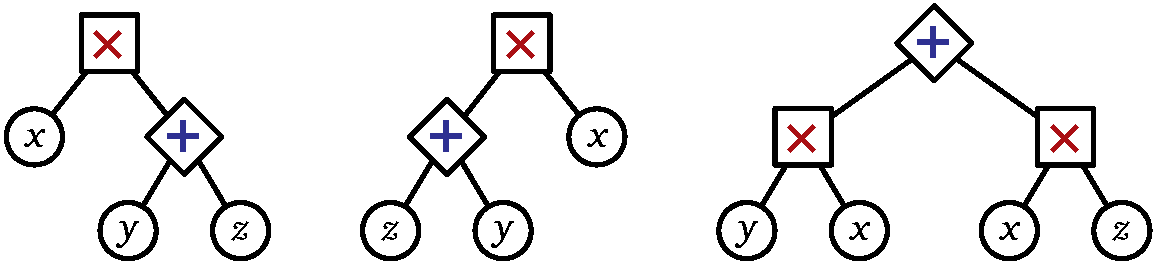
\includegraphics[height=0.75in]{Fig/exp-trees}\\
Three equivalent expression trees.  Only the third tree is in normal form.
\end{inline}

Prove that for any arithmetic expression tree, there is an equivalent arithmetic expression tree in normal form.  \Hint{Be careful.  This is trickier than it looks.}


%----------------------------------------------------------------------
\item
Recall that a standard (Anglo-American) deck of 52 playing cards contains 13 cards in each of four suits: spades (\Spade), hearts (\Heart), diamonds (\Diamond), and clubs (\Club).  Within each suit, the 13 cards have distinct \emph{ranks}: 2, 3, 4, 5, 6, 7, 8, 9, 10, jack ($J$), queen ($Q$), king ($K$), and ace ($A$).  The ranks are ordered $2 < 3 < \cdots < 9 < 10 < J < Q < K < A$; thus, for example, the jack of spades has higher rank thank the eight of diamonds.

\href{http://www.youtube.com/watch?v=UWvRorX0KhQ}{Professor Jay} is about to perform a public demonstration with two decks of cards, one with red backs (`the red deck') and one with blue backs (`the blue deck').  Both decks lie face-down on a table in front of Professor Jay, \href{http://www.youtube.com/watch?v=6LYjMHzQ_oU}{shuffled} uniformly and independently.  Thus, in each deck, every permutation of the 52 cards is equally likely.

To begin the demonstration, Professor Jay turns over the top card from each deck.  Then, while he has not yet turned over a three of clubs (3\Club), the good Professor hurls the two cards he just turned over into the \href{http://www.youtube.com/watch?v=k1ZGIN0UqJE}{thick, pachydermatous outer melon layer} of a nearby watermelon (that most prodigious of household fruits) and then turns over the next card from the top of each deck.  Thus, if {3\Club} is the last card in both decks, the demonstration ends with 102 cards embedded in the watermelon.

\begin{enumerate}
\item
What is the \emph{exact} expected number of cards that Professor Jay hurls into the watermelon?

\item
For each of the statements below, give the \emph{exact} probability that the statement is true of the \EMPH{first} pair of cards Professor Jay turns over.
\begin{enumerate}
\item
Both cards are threes.
\item
One card is a three, and the other card is a club.
\item
If (at least) one card is a heart, then (at least) one card is a diamond.
\item
The card from the red deck has higher rank than the card from the blue deck.
\end{enumerate}

\item
For each of the statements below, give the \emph{exact} probability that the statement is true of the \EMPH{last} pair of cards Professor Jay turns over.
\begin{enumerate}
\item
Both cards are threes.
\item
One card is a three, and the other card is a club.
\item
If (at least) one card is a heart, then (at least) one card is a diamond.
\item
The card from the red deck has higher rank than the card from the blue deck.
\end{enumerate}
\end{enumerate}
Express each of your answers as rational numbers in simplest form, like $123/4567$.  \EMPH{Do not submit proofs}---just a list of rational numbers---but you should do them anyway, just for practice.


%----------------------------------------------------------------------

\end{enumerate}

\end{document}
